\documentclass[a4paper,12pt]{article}

\pdfminorversion=4

\usepackage[left=2.5cm,top=2.5cm,right=2.5cm,bottom=2.5cm]{geometry}

\usepackage[T1]{fontenc}
\usepackage[spanish]{babel}
\usepackage[utf8]{inputenc}

\usepackage[pdftex, breaklinks=false, colorlinks=true, linkcolor=black, anchorcolor=black, urlcolor=blue, citecolor=red]{hyperref}
\usepackage{graphicx}
\usepackage{times}
\usepackage{inconsolata}
\usepackage{float}
\usepackage{minted}

\usemintedstyle[console]{vs}

\newminted[bashcode]{console}{} % tango vs
\newminted{python}{}
\newminted{json}{}


\graphicspath{{./img/}}

%\usepackage{framed}

% \usepackage{amsfonts}
% \usepackage{amssymb}
% \usepackage{amsthm}
% \usepackage{amsmath}
% \usepackage{array}
% \usepackage{caption}
% \usepackage{color}
% \usepackage[mirror]{crop} %<--------------LOL
% \usepackage{eurosym} %para el simbolo del euro
% \usepackage{fancybox}
% \usepackage[Rejne]{fncychap}% Sonny, Glenn, Lenny, Conny, Rejne, Bjarne
% \usepackage{float}
% \usepackage{fullpage}
% \usepackage{graphicx}
% \usepackage{multirow}
% \usepackage{pifont}
% \usepackage{stmaryrd}
% \usepackage{supertabular}
% \usepackage[dotinlabels]{titletoc}
% \usepackage[all]{xy}
% \usepackage{wasysym}




%\usepackage{tikz}


%\usepackage{xxcolor}

%\usepackage{mathdesign}
%\usepackage{titlesec}


%\usepackage{estiloBase}
%\usepackage{colores}
%\usepackage{bera}
\usepackage{comandos}

% \usepackage{setspace}

% \usepackage{calc}

% \addto\captionsspanish{
% \renewcommand\bibname{Bibliografía y referencias}
% }

\def \titulo{Sitic: framework para generar páginas web estáticas}
\def \autor{Alumno: José Jesús Marente Florín\\Tutor: José Miguel Mota Macías}
\def \fecha{Septiembre de 2017}

\usepackage{parskip}
\usepackage{abstract}

\begin{document}
\portada

\vspace{0.25cm}

\begin{abstract}
\textbf{Sitic} es un framework generador de sitios web estáticos. El usuario escribirá
los contenidos de la web en ficheros de textos plano y la
herramienta generará una web completamente estática a partir de estos ficheros,
transformándolos en HTML.

Entre otras características, la herramienta usa un sistema de plantillas que permite al
usuario personalizar la forma en la que se mostrarán todos los contenidos. Así mismo,
permitirá al usuario definir los atributos básicos de cada página y ofrecerá otras
posibilidades como generación de menús o generación de RSS.

Estará totalmente desarrollado usando el lenguaje de programación Python~\cite{python} y usará como
base el sistema de plantillas Jinja~\cite{jinja}. \\

\textbf{Palabras clave:} Internet, Web, HTML, Python, Jinja.

\end{abstract}


% \vspace{0.5cm}

\section{Introducción}

\subsection{Contexto y motivación}

La idea de desarrollar este proyecto surge a raíz de usar otras herramientas con un objetivo
parecido, pero que no llegaban a satisfacer todas las funcionalidads que necesitaba, viéndote obligado
a suplirlas con otras herramientas que no eran totalmente compatibles con las originales.

En noviembre de 2015 forme parte en el desarrollo de una página web totalmente estática con información
bastante importante a la que accederían personas de distintos idiomas. Para el desarrollo de la web mencionada,
se usó Hugo~\cite{hugo}, uno de los generadores estáticos más conocidos. Pero a pesar de ser uno de los más usados,
la herramienta carecía de funcionalidades que considerábamos totalmente imprescindibles en el desarrollo
de una plataforma tan importante.

De ahí nace la motivación para intentar desarrollar una herramienta que aunque siga los mismos principios,
añada funcionalidades de las que las herramientas actuales carecen y no tiene pensado añadir en un futuro
próximo.

También he de añadir que tras conocer abiertamente el mundo del Software libre, gracias a la importancia
que se le presta en la Universidad de Cádiz. Se decidió que el proyecto fuera software libre bajo
licencia GPL. Y así cualquier persona interesada en el proyecto y en el software libre
en general, pudiera usar los recursos del proyecto o colaborar libremente.

\subsection{Objetivos}

A la hora de definir los objetivos de un sistema, podemos agruparlos en dos tipos
diferentes: funcionales y transversales. Los primeros se refieren a qué debe hacer
la herramienta que vamos a desarrollar, e inciden directamente en la experiencia del
usuario y de potenciales desarrolladores.

Por otro lado, los objetivos transversales son aquellos invisibles al usuario final,
pero que de forma inherente actúan sobre el resultado final de la aplicación y
sobre la experiencia de desarrollo de la misma.

\subsubsection{Funcionales}
\begin{itemize}
\item Crear una herramienta que permita a los usuarios crear una web completamente estática
con todas las funcionalidades que una web normal y dinámica tienen.
\item Dar la posibilidad a los usuarios de personalizar en la medida de todo lo posible la configuración
inicial de la herramienta de forma que puedan adaptar lo máximo posible a sus necesidades.
\item Dar la posibilidad que cualquier usuario medio Linux pueda crear una web desde cero sin tener
ningún conocimiento de programación o de servidores web.
\end{itemize}

\subsubsection{Transversales}
\begin{itemize}
\item Aplicar mis conocimientos sobre el desarrollo web en general.
\item Adquirir soltura en el uso del lenguaje de programación Python en herramientas de terminal.
\item Utilizar un enfoque de análisis, diseño y codificación orientado a objetos,
de una forma lo más clara y modular posible, para permitir ampliaciones y
modificaciones sobre la aplicación por terceras personas.
\item Hacer uso de herramientas básicas en el desarrollo de software, como son los
sistemas de control de versiones para llevar un control realista del desarrollo
del software, así como hacer de las veces de sistema de copias de seguridad.
\end{itemize}

\subsection{Planificación}

El proyecto se ha desarrollado siguiendo un calendario basado en fases, utilizando un modelo
de desarrollo iterativo incremental.

\subsubsection{Fase inicial}

La primera fase consistió en plantear la idea del proyecto, con la ayuda del tutor. Tras plantear
varios enfoques, se decidió realizar este proyecto debido a las motivaciones escritas anteriormente.

También se pensó en qué lenguaje se desarrollaría el proyecto, así como las principales bibliotecas que
se usarían durante la realización del mismo, priorizando siempre opciones libres. Finalmente se optó por
utilizar el lenguage Python por su documentación, comunidad y amplia biblioteca estándar.

\subsubsection{Fase de análisis}

Esta etapa está dividida principalmente en las dos partes siguiente:

\begin{itemize}
\item Especificación de los requisitos: estudio de los requisitos que deberá cumplir el proyecto.
\item Recursos necesarios: recursos necesarios que deberemos usar durante el desarrollo del proyecto.
\end{itemize}

\subsubsection{Fase de aprendizaje}

Aunque ya había realizado otros proyectos en Python, decidí dedicarle tiempo a perfeccionar mis conocimientos
sobre el lenguaje, así como de la librería estándar y las posible bibliotecas que me serían útiles en el desarrollo.

Esta fase se caracterizó por intentar entender código ya escrito así como leer tutoriales y documentación
oficial. Se podría dividir en estas etapas:

\begin{itemize}
\item \textbf{Perfeccionamiento del lenguaje Python}: investigar sobre el propio lenguaje, biblioteca estándar
así como metodologías a utilizar.
\item \textbf{Aprendizaje de otras bibliotecas}: investigar bibliotecas externas desarrolladas por la comunidad y
que podrían ser útiles en el desarrollo.
\item \textbf{Investigar sobre lenguajes de marcado}: dado que el usuario escribirá el contenido de la web en ficheros
de texto plano y haciendo uso de lenguajes de marcado. Invertí tiempo en ver cuáles eran los más usados, para así poder
darles soporte en la herramienta.
\end{itemize}

\subsubsection{Fase de desarrollo}

Tras la consecución de las etapas anteriores, se comenzó el desarrollo del proyecto. Esta etapa del desarrollo
es la más extensa de todas, como es comprensible. Y me fue posible llevarla a cabo gracias a los
prototipos que iba implementando conforme aprendía.

\begin{itemize}
\item \textbf{Generador básico}: Como primer paso se realizó un generador básico de ficheros a partir
de ficheros de texto plano. Esto incluía la generación estructural de toda la web resultante.
\item \textbf{Adaptar sistema de plantillas}: Otro de los aspectos más importantes fue adaptar el sistema
de plantillas usado (Jinja) con el motor de generación de forma que los HTML generados fueran totalmente
personalizables por los usuarios.
\item \textbf{Mejor de output}: Al ser una herramienta que se ejecuta por la linea de comandos, se invirtió
bastante tiempo en que el output ofrecido al usuario fuera realmente verbose y útil, dando información relevante.
\item \textbf{Internacionalización}: Sistema de internacionalización fácil e intuitivo de usar, que permitirá al usuario
escribir plantillas HTMLs una única vez para todos los idiomas configurados.
\item \textbf{Ampliación de funcionalidades}: una vez que ya se había desarrollado toda las funcionalidades básicas,
se dedico tiempo a mejorar las ya existentes, así como a implementar nuevas.
\end{itemize}


\subsubsection{Pruebas y correcciones}

Una de las etapas más importantes del desarrollo de cualquier proyecto. Esta etapa se realizó en paralelo
a la de desarrollo, ya que conforme se implementaron nuevas funcionalidades, se iban probando exhaustivamente
bajo el contexto de las distintas situaciones que pudiera darse, hasta obtener el comportamiento
esperado.

\subsubsection{Redacción de la memoria}

La redacción de la memoria se ha redactado conforme se iba avanzando en el desarrollo del proyecto.
Pero tras la finalización de éste, se le ha dedicado más tiempo a su finalización, corrigiendo puntos que
finalmente no se han adecuado al producto final.

\subsubsection{Diagrama de Gantt}

\paragraph{}
Diagrama de Gantt de la planificación comentada (Figura \ref{fig:gantt}).

\begin{figure}[htbp]
    \centering
    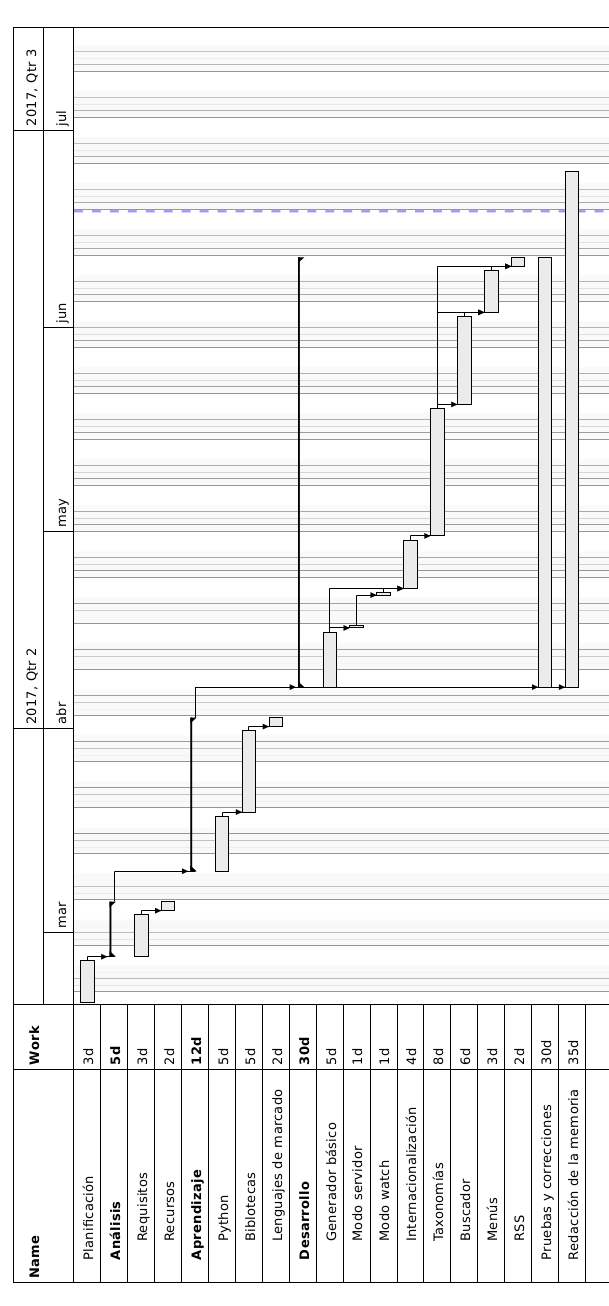
\includegraphics[width=0.7\textwidth]{img/diagrama_gantt}
    \caption{Diagrama de Gantt}
    \label{fig:gantt}
\end{figure}

%%%%%%%%%%%%%%%%%%%%%%%%%%%%%%%%%%%%%%%%%%%%%%%%%%%%%%
%%%%%%%%%%%%%%%%%%%%%%%%%%%%%%%%%%%%%%%%%%%%%%%%%%%%%%

\section{Descripción}

Sitic es un framework para hacer sitios web de uso general. Técnicamente hablando, Sitic es un generador de sitios web estáticos.
A diferencia de otros sistemas que genera dinámicamente una página cada vez que un visitante la solicita, Sitic crea el sitio
una única vez,
cuando creas su contenido. Dado que los sitios web se ven con mucha más frecuencia de lo que se edita.

Los sitios construidos con Sitic son bastante más rápidos y seguros que un sitio generado de forma dinámica.
Se pueden alojar en cualquier lugar, incluyendo GitHub Pages, Google Cloud Storage o Amazon
S3 entre otros. Los sitios de Sitic se ejecutan sin depender de tiempos de ejecución costosos como Ruby, Python
o PHP y sin dependencia de ninguna base de datos, en lo que se refiere al lado del servido, solo el tiempo
que el navegador del usuario necesite para descargar la página visitada. En referencia al lado
del cliente como puede ser el ejecución del Javascript que el usuario haya desarrollado, dependerá del navegador y
equipo del usuario.

\subsection{Diferencia con los generadores dinámicos}

Los generadores de sitios web generan contenidos en ficheros HTML. La mayoría son "generadores dinámicos".
Esto significa que el servidor HTTP (que es el programa que se ejecuta en su sitio web con el que el navegador del
usuario habla) ejecuta el generador para crear un nuevo fichero HTML cada vez que un usuario desea ver una página.

Crear la página de forma dinámica significa que la máquina que aloja el servidor HTTP tiene que tener suficiente
memoria y CPU para ejecutar el generador de forma eficaz durante todo el día. Si no, entonces el usuario tiene que
esperar a que la página se genere.

Nadie quiere que los usuarios esperen más de lo necesario, por lo que los generadores de sitios dinámicos programaron
sus sistemas para almacenar en caché los ficheros HTML. Cuando un fichero se almacena en caché, una copia se
almacena temporalmente en el equipo. Es mucho más rápido que el servidor envíe esa copia la próxima vez que
se solicite la página en lugar generarla desde cero.

Sitic intenta llevar el almacenamiento en caché un paso más allá. Todos los ficheros HTML se representan en su máquina.
Puede revisar los ficheros antes de copiarlos en la máquina que aloja el servidor HTTP. Dado que los ficheros HTML
no se generan dinámicamente, decimos que Sitic es un "generador estático".

No tener que ejecutar la generación de HTML cada vez que se recibe una petición tiene varias ventajas. Entre ellas,
la más notable es el rendimiento, los servidores HTTP son muy buenos en el envío de ficheros. Tan bueno que puede
servir eficazmente el mismo número de páginas con una fracción de memoria y CPU necesaria para un sitio dinámico.

Sitic tiene dos componentes para ayudarle a construir y probar su sitio web. El que probablemente usará más a menudo es el
servidor HTTP incorporado. Cuando ejecuta el servidor, Sitic procesa todo su contenido en ficheros HTML y luego ejecuta
un servidor HTTP en su máquina para que pueda ver cómo son las páginas.

El segundo componente se utiliza una vez que el sitio esté listo para ser publicado.
Ejecutar Sitic sin ninguna acción reconstruirá su sitio web completo utilizando la configuración \texttt{base\_url}
del fichero de configuración de su sitio. Eso es necesario para que sus enlaces de página funcionen correctamente
con la mayoría de las empresas de alojamiento.

\subsection{Características principales}

En términos técnicos, Sitic toma un directorio fuente de ficheros
y plantillas y los usa como entrada para crear un sitio web completo.

Sitic cuenta con las siguientes características:

\paragraph{General}

\begin{itemize}
\item Tiempos de generación rápidos
\item Fácil instalación
\item Posibilidad de alojar su sitio en cualquier lugar
\end{itemize}

\paragraph{Organización}

\begin{itemize}
\item Organización sencilla
\item Soporte para secciones
\item URL personalizables
\item Soporte para taxonomías configurables que incluyen categorías y etiquetas.
\item Capacidad de clasificar el contenido como se desee
\item Generación automática de tabla de contenidos
\item Creación dinámica de menús
\item Soporte de URLs legibles
\end{itemize}

\paragraph{Contenido}

\begin{itemize}
\item Soporte nativo para contenido escrito en Markdown~\cite{markdown}, Textile~\cite{textile} y Reestructured text~\cite{restructuredtext}
\item Soporte para internacionalización
\item Soporte para especificar metadatos, usando TOML~\cite{toml} y YAML~\cite{yaml} como formatos, en los contenidos
\item Páginas completamente personalizables
\end{itemize}

%%%%%%%%%%%%%%%%%%%%%%%%%%%%%%%%%%%%%%%%%%%%%%%%%%%%%%
%%%%%%%%%%%%%%%%%%%%%%%%%%%%%%%%%%%%%%%%%%%%%%%%%%%%%%

\section{Desarrollo del sistema}

El desarrollo de la plataforma web de \textbf{Sitic} supuso un reto por el cúmulo de tecnologías
involucradas y las cuestiones que surgieron durante la implementación. El stack tecnológico
utilizado se detalla a continuación:

\begin{figure}[htbp]
    \centering
    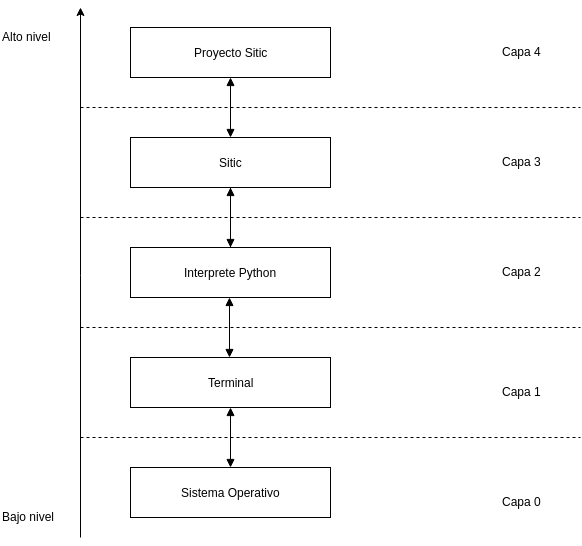
\includegraphics[width=0.9\textwidth]{img/arquitectura_logica}
    \caption{Arquitectura lógica}
    \label{fig:arquitectura-logica}
\end{figure}

\begin{itemize}
\item Como lenguaje principal de desarrollo se ha usado \textbf{Python}~\cite{python} por su
documentación, comunidad y amplia biblioteca estándar.

\item Para el motor de plantillas quse ha usado \textbf{Jinja2}~\cite{jinja}, es un motor de
plantillas completo para Python. Cuenta con soporte unicode completo, un entorno de ejecución de
espacio de trabajo integrado opcional, ampliamente utilizado y licenciado por BSD.

\item Los lenguajes de marcados soportados para que el usuario pueda escribir los contenidos de las web
han sido \textbf{Markdown}~\cite{markdown}, \textbf{Textile}~\cite{textile} y
\textbf{Reestructured text}~\cite{restructuredtext}, a pesar de que el primer de ellos nombrados, es el mas usado
debido a sus sencillez, se decidión que el sistema soportara más de uno de forma que el usuario pudiera usar aquel
con el que se sintiera más cómodo.

\item La forma en la que el usuario pudiera configurar información extra en los ficheros de contenidos, se decidió usar
    los formatos \textbf{YAML}~\cite{toml} y \textbf{TOML}~\cite{yaml}, por su simplicidad y flexibilidad.
\end{itemize}

Además de las mencionadas, se han utilizado muchas otras tecnologías y herramientas de apoyo
al desarrollo, que se detallan más profundamente en la memoria del proyecto.

\subsection{Detalles implementación}

\subsubsection{Estructura de ficheros}

Uno de los primeros retos a la hora de la implementación, era ofrecer al usuario una forma sencilla de dividir
el contenido de los ficheros y los metadatos de estos.

Para que fuera sencillo tanto para los usuario, como para la herramienta poder diferencias esas dos partes
de forma inequívoca, se decidió que los ficheros de contenidos usará delimitadores que marcaran que
parte eran metadatos y debía ser tratados como tal y que parte era el contenido real del fichero.

Dado que el sistema ofrece escribir los metadatos en dos formatos, \texttt{YAML} y \texttt{TOML}, se decidió que cada
uno tuviera su propio carácter delimitador:

\begin{itemize}
    \item El formato \texttt{TOML} usaría el carácter +.
    \item El formato \texttt{YAML} usaría el carácter -.
\end{itemize}

A continuación se puede ver un ejemplo de un fichero de contenido \texttt{Markdown}~\cite{markdown} con los metadatos en formato
\texttt{TOML}:

\begin{verbatim}
++++++++++++++++
title='Post 1'
tags=['tag1', 'tag2']
description="Post 1 description"
++++++++++++++++

## Variarum loricaeque

Lorem markdownum mihi. Avidoque doloris stabit; omen turaque est, ante ergo
nostraque, tibi.

    cpl_monitor_clean += html_window(management_ddl * 3, hacker);
    ccd -= -3;
    alignment_sdram += netbios_optical_party.webHardening(recycle_horizontal(5,
            networkCmsOpen, bandwidth_computer - text), -1);

## Curam vires adhuc domum

Tendere posuisse fatorum pharetras e diversis *lacertos*: ius cum vacuaque denos
quem, ausa transit puero. Undique foret et restatque supremaque accessi utile
mollire [bracchia Othryn](http://www.ratibus.net/curvavit.html) manumque; vimque
exprobravit sola ferrum diverso inania terramque. Qui illic et Romulus, ad erat
Pergama daedalus annis, fudit.

\end{verbatim}

Internamente el sistema automáticamente divide el contenido del fichero en dos partes y las procesa por separado.
A continuación se puede ver el fragmento de código que se encarga de realizar dicha tarea:

\subsubsection{Buscador}

Hoy en día, cualquier sitio web con un número de páginas elevado, necesita un
buscador con el que se puedan encontrar los contenidos de forma sencilla.

Dado que \texttt{Sitic} genera un sitio web completamente estático, lo que implica que no tenemos ningún
servidor al que hacerle peticiones con los términos que se desean buscar, se decidió implementar
una búsqueda acorde a las características de la herramienta.

Para conseguirlo, la implementación consistía en varias partes, la primera de ellas, generar un índice de contenidos
en un fichero JSON que incluyera todos los contenidos publicados.

EL JSON resultante tendría el siguiente formato:

\begin{jsoncode}
[
    {
        "content": "Variarum loricaeque\nLorem markdownum mihi...",
        "title": "Post 1",
        "url": "/blog/post1"
    },
    {
        "content": "Variarum loricaeque\nLorem markdownum mihi...",
        "title": "Post 2",
        "url": "/blog/post2"
    },
    {
        "content": "Variarum loricaeque\nLorem markdownum mihi...",
        "title": "Post 6",
        "url": "/blog/post6"
    }
]
\end{jsoncode}

Este fichero se añadiría a la carpeta del sitio generado.

La tercera parte requería implementar la lógica necesaria en \texttt{Javascript} que usara el índice generado
y devolviera los resultados encontrados. Para ello se hizo uso de la biblioteca \texttt{Lunr.js} para
\texttt{Javascript} que permite realizar búsquedas en índices adaptados previamente a su formato.

La tercera y última parte de la implementación consiste en que el usuario pueda de forma sencilla añadir dicho buscador en
su web, para ello, se debe añadir un formulario con un id específico que el código \texttt{Javascript} anteriormente
comentado consultará y por último generar una plantilla llamada \texttt{search-results.js} con un bloque
determinado donde se mostrarán los resultados de la búsqueda.

\subsection{Verificación y pruebas}

El diseño de casos de pruebas para un proyecto de las características de \emph{Sitic}
es algo complicado, ya que estamos en un escenario simulando como interactúan muchísimos
elementos entre sí. Pero las pruebas son algo necesario si deseamos un software con una
calidad aceptable.

Todos los módulos que componen la aplicación han sido probados individualmente, como pueden
ser aquellos módulos encargados de la gestión de idiomas, generación de contenidos o categorización.

También se realizaron pruebas de integración, ya que había módulos, una vez probado en solitario,
debían realizar distintas acciones junto con otros módulos.

Otras pruebas que se realizaron fueron de generación, tanto yo como
personas ajenas al desarrollo de proyecto probaron el
mismo ofreciendo sus opiniones sobre aspectos que deberían ser modificados o
errores que aparecían a lo largo de la ejecución y en el resultado obtenido.

En definitiva, la organización de los casos de pruebas fue la siguiente:

\begin{enumerate}
    \item Tras finalizar la implementación de cada módulo, se realizaban pruebas unitarias sobre estos.
    \item A medida que distintos módulo que anteriormente probados individualmente, debían colaborar entre ellos, se
    llevaban a cabo pruebas de integración.
    \item Con las distintas versiones usables se realizaban pruebas de generación.
\end{enumerate}

\subsubsection{Pruebas unitarias}

Esta pruebas se realizaron junto a la fase de implementación, conforme se implementaban nuevos módulos necesarios para la aplicación
se realizaban pruebas individuales sobre estos módulos. De esta forma se buscaban todos los caminos posibles que podría dar cada
módulo, teniendo en cuenta aquellos que fueran más predispuesto a fallos.

De esta forma todas las sentencias se ejecutaban como mínimo una vez y los posibles fallos se encontraban de una forma más sencilla.
Por lo que también eran más fácil localizar donde estaba el problema y afrontar la solución de este.

\subsubsection{Pruebas de integración}

Conforme aparecían nuevos módulos, cuya implementación era necesaria y a su vez estos requerían el uso de otro módulos que
posteriormente habían sido probados individualmente, se realizaban pruebas de integración entre dichos módulos.

Conforme se avanzaba en el desarrollo, se realizaban pruebas de integración a mayor escala. No solo entre módulos
del mismo sistema, sino entre varios sistemas.

Una de las mejores formas que se pesaron para realizar este tipo de pruebas, fue desarrollar una web que usara todos los elementos
que se iban implementando.

\subsubsection{Pruebas de aceptación}

Conforme se avanzaba en el desarrollo del proyecto y se conseguían versiones estables del mismo, se
envíaban estas versiones, junto con el manual del proyecto, a un grupo de usuarios con los conocimientos
necesarios, capaces de interpretar los requerimientos especificados por los futuros usuarios de la herramienta.

El manual se iba actualizando con las nuevas funcionalidades que se iban añadiendo. De forma que
los usuarios pudieran identificar y probar correctamente todas las características de la herramienta.

Cada uno de estos usuarios devolvía un pequeño informe sobre la herramienta, en la que detallaban los distintos
problemas que se habían encontrado, errores que necesitaban ser corregidos y su opinión sobre
funcionalidades, indicando cuales podría ser ampliadas para que fueran más útiles o más sencillas de usar.

Con cada uno de estos informes, se trabajaba para mejorar la herramienta en la siguientes versiones, dando
prioridad a aquellas que se consideraban más críticas.

\subsubsection{Pruebas de generación}

Cada vez que estaban disponibles nuevas versiones estables de la herramienta, se pedían la ayuda a personas,
totalmente ajenas al desarrollo, que probaran las distintas versiones disponibles. De esta forma cada uno
de los colaboradores daba su opinión sobre  distintos aspectos como la usabilidad, dificultad, respuesta o eficiencia.
Tras recopilar la información que todos ellos proporcionaron, se procedía a realizar los ajustes
necesarios a los distintos parámetros requeridos.

Entre los distintos aspectos a probar que se le recomendaban a los
colaboradores que hicieran especial hincapié, son los siguiente:

\begin{itemize}
\item \textbf{Internacionalización}: definición de varios idiomas con contenidos divididos, así como pruebas de generar
los mismos contenidos sin ningún idioma configurado.
\item \textbf{Urls de ficheros}: definir distintas urls en los ficheros, comprobando que la generación se la ruta
se generaba de forma correcta, en función de la rutas definidas
\item \textbf{Paginación}: configurar distintos valores para la paginación de elementos por página, así como la desactivación
del mismo, comprobando que se generaban tantas páginas estáticas por sección/taxonomías como páginas debería de tener.
\item \textbf{Menús}: Definición de menús con elementos estáticos y dinámicos.
\item \textbf{Categorización}: definir distintas taxonomías y mezclarlas entre los idiomas, comprobando finalmente que cada
contenido se había organizado de la forma correcta.
\end{itemize}


%%%%%%%%%%%%%%%%%%%%%%%%%%%%%%%%%%%%%%%%%%%%%%%%%%%%%%
%%%%%%%%%%%%%%%%%%%%%%%%%%%%%%%%%%%%%%%%%%%%%%%%%%%%%%

\section{Conclusiones}

Durante el transcurso del desarrollo de Sitic, y sobre todo al término del mismo,
se han obtenido unas conclusiones y unos resultados, tanto de forma personal
como para con la comunidad, que intentaremos reflejar en este capítulo.

\subsection{Resumen de objetivos}

Es evidente que su realización no me ha dejado indiferente. No ha sido fácil construir una idea
clara sobre lo que se quería hacer. Así como solucionar los distintos problemas que han ido apareciendo
a lo largo del desarrollo de este.

También decir que el proyecto me ha ocupado bastante más tiempo del esperado en un principio. Tuve
muchos problemas y alguna que otra duda en algunas fases del desarrollo de proyecto, que me tuvieron
bloqueado durante un tiempo hasta encontrar la solución más adecuada para estos. A pesar de todo,
estoy muy satisfecho con el resultado que se ha obtenido.

Se puede decir que el proyecto goza de buena calidad. Se ha intentado hacer un software sencillo,
intuitivo y fácil de usar.

\subsection{Conclusiones personales}

Durante el desarrollo del proyecto se han aprendido muchísimas cosas: como hacer distintas ramas de
desarrollo, plantear y crear calendarios, usar las herramientas adecuadas, hacer decisiones importantes
para el desarrollo de este, documentación del código, organización, etc. Ya que durante la carrera se
han realizado distintas prácticas y trabajos de complejidad, pero nada con el tamaño y duración que
requiere un Proyecto de fin de carrera. Una vez finalizado, creo que tengo la experiencia necesaria
para afrontar otro proyecto con buenos resultados.

Puedo decir que he profundizado y consolidado bastante en el lenguaje de programación Python.
Además he obtenido más práctica a la hora de manejar bibliotecas
externas, así como entender su documentación e integrarlas en un proyecto.

En definitiva, este proyecto me ha hecho madurar como persona, estudiante y profesional. He aprendido a buscar
bibliografía, opiniones en otras personas, compartir ideas, seguir un horario, cumplir una fechas de
entrega y enfrentarme a un proyecto de estas características.

\subsection{Mejoras y ampliaciones}

Las posibles mejoras y ampliaciones que se podrían añadir al proyecto en futuras versiones, se comentan
a continuación:

\begin{itemize}
    \item \textbf{Soporte Filtros/funciones propias} de forma que cada usuario puede personalizar aún mas
    funciones a usar en las plantillas.
    \item \textbf{Método watch que recargue automáticamente el navegador}: permitir que el modo watch recargue
    automáticamente el navegador cuando se detecte algún cambio.
    \item \textbf{Permitir temas}: permitir la creación de temas, es decir, poder usar temas definidos
    por otros usuarios y únicamente preocuparte por la redacción del contenido.
    \item \textbf{Permitir fichero con contenido para taxonomía}: permitir definir metadatos en las taxonomías
    tal y como se puede hacer en los contenidos y secciones.
    \item \textbf{Permitir publicar un solo idioma}: no verse obligado a generar el sitio completo y podre generar
    un único idioma o página.
\end{itemize}

\bibliographystyle{hispa-annote}
\bibliography{bibliografia}

\vspace{0.75cm}

\begin{center}
{\footnotesize Este documento se halla bajo la licencia FDL de GNU (Free Documentation
  License)\\ \url{http://www.gnu.org/licenses/fdl.html} }
\end{center}

\end{document}
